\documentclass{article}
\usepackage{graphicx}
\usepackage[margin=1.5cm]{geometry}
\usepackage{amsmath}

\begin{document}

\title{Tuesday Reading Assessment: Unit 4, AC Generators}
\author{Prof. Jordan C. Hanson}

\maketitle

\section{Memory Bank}

\begin{itemize}
\item $\epsilon = -N \Delta \phi_m /\Delta t$ ... Faraday's Law
\item $\phi_m = \vec{B} \cdot \vec{A} = BA \cos(\theta)$ ... Definition of magnetic flux
\item $\epsilon(t) = \epsilon_0 \sin(\omega t)$ ... AC voltage generated by generator.
\item $P_{max} = V_{max}^2/R$ ... Max power of an AC generator.
\item $P_{ave} = \frac{1}{2} P_{max}$ ... Average power of an AC generator.
\end{itemize}

\section{AC Generators}

\begin{enumerate}
\item Consider Fig. \ref{fig:acgen}.  Suppose that the angle between the area vector and the magnetic field is $\theta = \omega t$.  (a) Show that
\begin{equation}
\phi(t) = BA\cos(\omega t) \label{eq:ac}
\end{equation}
(b) Given Eq. \ref{eq:ac}, it turns out that the voltage generated in the loop is proportional to $\sin(\omega t)$ and $\omega$ itself.  That is,
\begin{equation}
\epsilon(t) = BA\omega \sin(\omega t)
\end{equation}
What is the voltage at a time $t = 1/240$ seconds, $\omega = 120\pi$ Hz, $B = 0.1$ T, and $A = 0.01$ m$^2$? (c) At what time is the voltage zero?
\begin{figure}[hb]
\centering
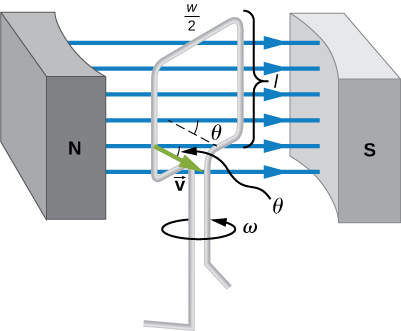
\includegraphics[width=0.35\textwidth]{acGen.jpeg}
\caption{\label{fig:acgen} A schematic of the concept of an AC generator.}
\end{figure}
\item Suppose the AC generator in Fig. \ref{eq:ac} has $V_0 = 12$ V so that $\epsilon(t) = V_0 \sin(\omega t)$.  If the AC generator pushes current through a resistance $R = 50\Omega$, what is the average power generated?
\end{enumerate}
\end{document}
